\begin{hcarentry}[updated]{GenI}
\label{geni}
\report{Eric Kow}%05/09
\makeheader

GenI is a surface realizer for Tree Adjoining Grammars. Surface
realization can be seen as the last stage in a natural language
generation pipeline. GenI in particular takes an FB-LTAG grammar and an
input semantics (a conjunction of first order terms), and produces the
set of sentences associated to the input semantics by the grammar.  It
features a surface realization library, several optimizations, batch
generation mode, and a graphical debugger written in wxHaskell.  It was
developed within the TALARIS project and is free software licensed under
the GNU GPL.

%**<img src="./GenI-main-screenshot.jpg">
%*ignore
\begin{center}
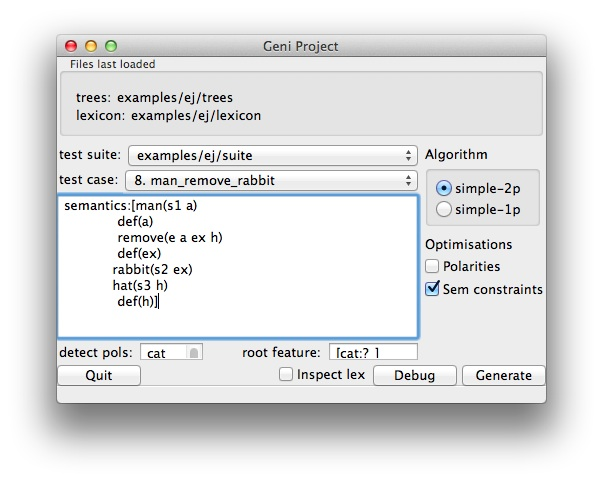
\includegraphics[width=0.47\textwidth]{html/GenI-main-screenshot.jpg}
\end{center}
%*endignore

%**<img src="./GenI-debugger-screenshot.jpg">
%*ignore
\begin{center}
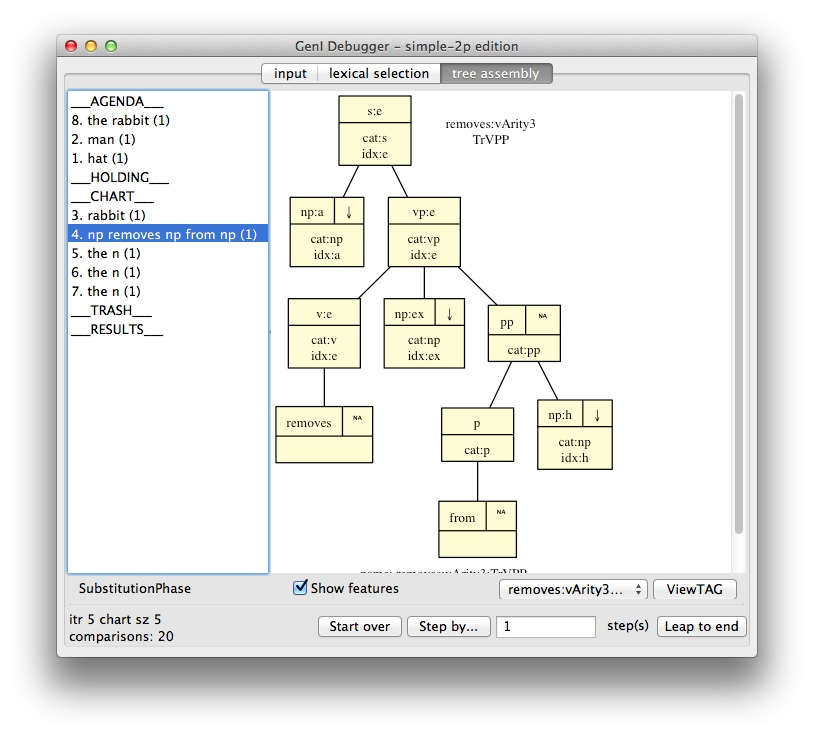
\includegraphics[width=0.47\textwidth]{html/GenI-debugger-screenshot.jpg}
\end{center}
%*endignore

GenI is available on Hackage, and can be installed via cabal-install.
Our most recent release of GenI was version 0.17.4, which offers
simplified installation with an optional graphical mode, and better help
text. For more information, please contact us on the geni-users mailing
list.

\FurtherReading
\begin{compactitem}
\item \url{http://trac.loria.fr/~geni}
\item Paper from Haskell Workshop 2006:

\url{http://hal.inria.fr/inria-00088787/en}
\item \url{http://websympa.loria.fr/wwsympa/info/geni-users}
\end{compactitem}
\end{hcarentry}
